% Created by tikzDevice version 0.10.1 on 2017-10-23 14:30:07
% !TEX encoding = UTF-8 Unicode
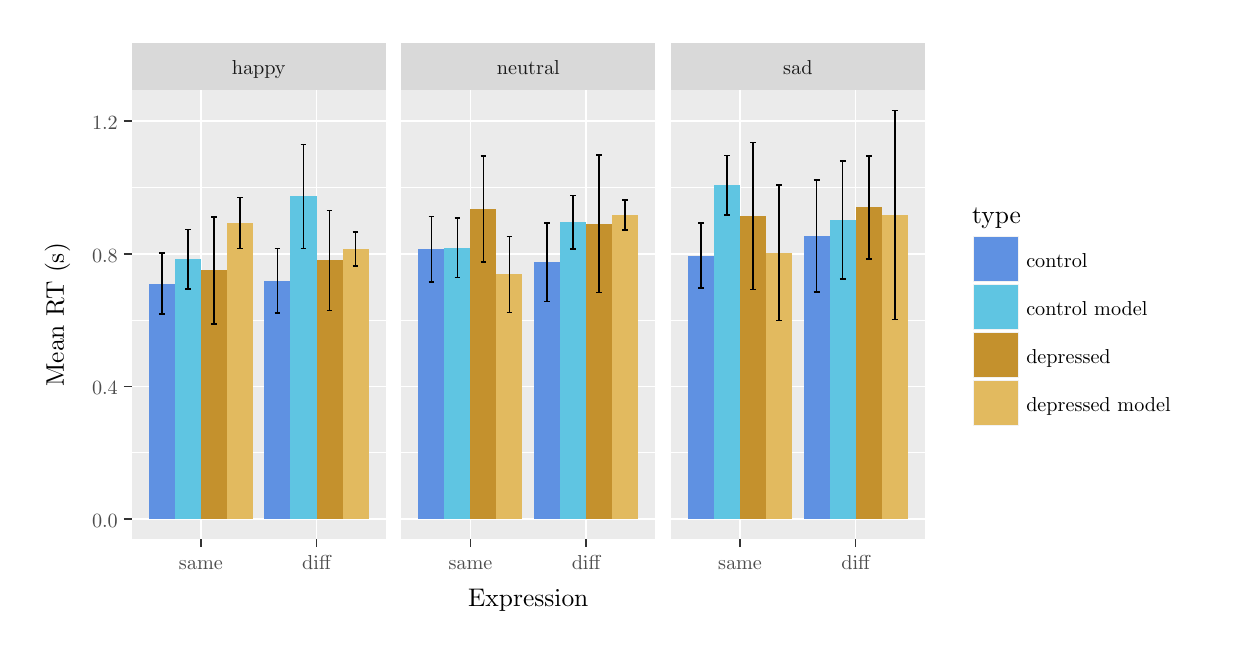
\begin{tikzpicture}[x=1pt,y=1pt]
\definecolor{fillColor}{RGB}{255,255,255}
\path[use as bounding box,fill=fillColor,fill opacity=0.00] (0,0) rectangle (433.62,216.81);
\begin{scope}
\path[clip] (  0.00,  0.00) rectangle (433.62,216.81);
\definecolor{drawColor}{RGB}{255,255,255}
\definecolor{fillColor}{RGB}{255,255,255}

\path[draw=drawColor,line width= 0.6pt,line join=round,line cap=round,fill=fillColor] ( -0.00,  0.00) rectangle (433.62,216.81);
\end{scope}
\begin{scope}
\path[clip] ( 37.53, 31.92) rectangle (129.44,194.25);
\definecolor{fillColor}{gray}{0.92}

\path[fill=fillColor] ( 37.53, 31.92) rectangle (129.44,194.25);
\definecolor{drawColor}{RGB}{255,255,255}

\path[draw=drawColor,line width= 0.3pt,line join=round] ( 37.53, 63.25) --
	(129.44, 63.25);

\path[draw=drawColor,line width= 0.3pt,line join=round] ( 37.53,111.15) --
	(129.44,111.15);

\path[draw=drawColor,line width= 0.3pt,line join=round] ( 37.53,159.06) --
	(129.44,159.06);

\path[draw=drawColor,line width= 0.6pt,line join=round] ( 37.53, 39.30) --
	(129.44, 39.30);

\path[draw=drawColor,line width= 0.6pt,line join=round] ( 37.53, 87.20) --
	(129.44, 87.20);

\path[draw=drawColor,line width= 0.6pt,line join=round] ( 37.53,135.10) --
	(129.44,135.10);

\path[draw=drawColor,line width= 0.6pt,line join=round] ( 37.53,183.01) --
	(129.44,183.01);

\path[draw=drawColor,line width= 0.6pt,line join=round] ( 62.60, 31.92) --
	( 62.60,194.25);

\path[draw=drawColor,line width= 0.6pt,line join=round] (104.37, 31.92) --
	(104.37,194.25);
\definecolor{fillColor}{RGB}{226,186,95}

\path[fill=fillColor] ( 72.00, 39.30) rectangle ( 81.40,146.21);
\definecolor{fillColor}{RGB}{196,145,45}

\path[fill=fillColor] ( 62.60, 39.30) rectangle ( 72.00,129.12);
\definecolor{fillColor}{RGB}{95,197,226}

\path[fill=fillColor] ( 53.20, 39.30) rectangle ( 62.60,133.11);
\definecolor{fillColor}{RGB}{95,145,226}

\path[fill=fillColor] ( 43.80, 39.30) rectangle ( 53.20,124.33);
\definecolor{fillColor}{RGB}{226,186,95}

\path[fill=fillColor] (113.77, 39.30) rectangle (123.17,136.84);
\definecolor{fillColor}{RGB}{196,145,45}

\path[fill=fillColor] (104.37, 39.30) rectangle (113.77,132.71);
\definecolor{fillColor}{RGB}{95,197,226}

\path[fill=fillColor] ( 94.97, 39.30) rectangle (104.37,155.83);
\definecolor{fillColor}{RGB}{95,145,226}

\path[fill=fillColor] ( 85.57, 39.30) rectangle ( 94.97,125.40);
\definecolor{drawColor}{RGB}{0,0,0}

\path[draw=drawColor,line width= 0.6pt,line join=round] ( 75.65,155.45) --
	( 77.74,155.45);

\path[draw=drawColor,line width= 0.6pt,line join=round] ( 76.70,155.45) --
	( 76.70,136.97);

\path[draw=drawColor,line width= 0.6pt,line join=round] ( 75.65,136.97) --
	( 77.74,136.97);

\path[draw=drawColor,line width= 0.6pt,line join=round] ( 66.25,148.40) --
	( 68.34,148.40);

\path[draw=drawColor,line width= 0.6pt,line join=round] ( 67.30,148.40) --
	( 67.30,109.84);

\path[draw=drawColor,line width= 0.6pt,line join=round] ( 66.25,109.84) --
	( 68.34,109.84);

\path[draw=drawColor,line width= 0.6pt,line join=round] ( 56.85,143.83) --
	( 58.94,143.83);

\path[draw=drawColor,line width= 0.6pt,line join=round] ( 57.90,143.83) --
	( 57.90,122.39);

\path[draw=drawColor,line width= 0.6pt,line join=round] ( 56.85,122.39) --
	( 58.94,122.39);

\path[draw=drawColor,line width= 0.6pt,line join=round] ( 47.45,135.34) --
	( 49.54,135.34);

\path[draw=drawColor,line width= 0.6pt,line join=round] ( 48.50,135.34) --
	( 48.50,113.31);

\path[draw=drawColor,line width= 0.6pt,line join=round] ( 47.45,113.31) --
	( 49.54,113.31);

\path[draw=drawColor,line width= 0.6pt,line join=round] (117.43,142.88) --
	(119.52,142.88);

\path[draw=drawColor,line width= 0.6pt,line join=round] (118.47,142.88) --
	(118.47,130.80);

\path[draw=drawColor,line width= 0.6pt,line join=round] (117.43,130.80) --
	(119.52,130.80);

\path[draw=drawColor,line width= 0.6pt,line join=round] (108.03,150.79) --
	(110.12,150.79);

\path[draw=drawColor,line width= 0.6pt,line join=round] (109.07,150.79) --
	(109.07,114.63);

\path[draw=drawColor,line width= 0.6pt,line join=round] (108.03,114.63) --
	(110.12,114.63);

\path[draw=drawColor,line width= 0.6pt,line join=round] ( 98.63,174.62) --
	(100.72,174.62);

\path[draw=drawColor,line width= 0.6pt,line join=round] ( 99.67,174.62) --
	( 99.67,137.03);

\path[draw=drawColor,line width= 0.6pt,line join=round] ( 98.63,137.03) --
	(100.72,137.03);

\path[draw=drawColor,line width= 0.6pt,line join=round] ( 89.23,137.02) --
	( 91.32,137.02);

\path[draw=drawColor,line width= 0.6pt,line join=round] ( 90.27,137.02) --
	( 90.27,113.79);

\path[draw=drawColor,line width= 0.6pt,line join=round] ( 89.23,113.79) --
	( 91.32,113.79);
\end{scope}
\begin{scope}
\path[clip] (134.94, 31.92) rectangle (226.85,194.25);
\definecolor{fillColor}{gray}{0.92}

\path[fill=fillColor] (134.94, 31.92) rectangle (226.85,194.25);
\definecolor{drawColor}{RGB}{255,255,255}

\path[draw=drawColor,line width= 0.3pt,line join=round] (134.94, 63.25) --
	(226.85, 63.25);

\path[draw=drawColor,line width= 0.3pt,line join=round] (134.94,111.15) --
	(226.85,111.15);

\path[draw=drawColor,line width= 0.3pt,line join=round] (134.94,159.06) --
	(226.85,159.06);

\path[draw=drawColor,line width= 0.6pt,line join=round] (134.94, 39.30) --
	(226.85, 39.30);

\path[draw=drawColor,line width= 0.6pt,line join=round] (134.94, 87.20) --
	(226.85, 87.20);

\path[draw=drawColor,line width= 0.6pt,line join=round] (134.94,135.10) --
	(226.85,135.10);

\path[draw=drawColor,line width= 0.6pt,line join=round] (134.94,183.01) --
	(226.85,183.01);

\path[draw=drawColor,line width= 0.6pt,line join=round] (160.00, 31.92) --
	(160.00,194.25);

\path[draw=drawColor,line width= 0.6pt,line join=round] (201.78, 31.92) --
	(201.78,194.25);
\definecolor{fillColor}{RGB}{226,186,95}

\path[fill=fillColor] (169.40, 39.30) rectangle (178.80,127.63);
\definecolor{fillColor}{RGB}{196,145,45}

\path[fill=fillColor] (160.00, 39.30) rectangle (169.40,151.27);
\definecolor{fillColor}{RGB}{95,197,226}

\path[fill=fillColor] (150.61, 39.30) rectangle (160.00,137.21);
\definecolor{fillColor}{RGB}{95,145,226}

\path[fill=fillColor] (141.21, 39.30) rectangle (150.61,136.66);
\definecolor{fillColor}{RGB}{226,186,95}

\path[fill=fillColor] (211.18, 39.30) rectangle (220.58,149.11);
\definecolor{fillColor}{RGB}{196,145,45}

\path[fill=fillColor] (201.78, 39.30) rectangle (211.18,146.00);
\definecolor{fillColor}{RGB}{95,197,226}

\path[fill=fillColor] (192.38, 39.30) rectangle (201.78,146.44);
\definecolor{fillColor}{RGB}{95,145,226}

\path[fill=fillColor] (182.98, 39.30) rectangle (192.38,131.99);
\definecolor{drawColor}{RGB}{0,0,0}

\path[draw=drawColor,line width= 0.6pt,line join=round] (173.06,141.34) --
	(175.15,141.34);

\path[draw=drawColor,line width= 0.6pt,line join=round] (174.10,141.34) --
	(174.10,113.93);

\path[draw=drawColor,line width= 0.6pt,line join=round] (173.06,113.93) --
	(175.15,113.93);

\path[draw=drawColor,line width= 0.6pt,line join=round] (163.66,170.43) --
	(165.75,170.43);

\path[draw=drawColor,line width= 0.6pt,line join=round] (164.70,170.43) --
	(164.70,132.11);

\path[draw=drawColor,line width= 0.6pt,line join=round] (163.66,132.11) --
	(165.75,132.11);

\path[draw=drawColor,line width= 0.6pt,line join=round] (154.26,147.93) --
	(156.35,147.93);

\path[draw=drawColor,line width= 0.6pt,line join=round] (155.31,147.93) --
	(155.31,126.48);

\path[draw=drawColor,line width= 0.6pt,line join=round] (154.26,126.48) --
	(156.35,126.48);

\path[draw=drawColor,line width= 0.6pt,line join=round] (144.86,148.52) --
	(146.95,148.52);

\path[draw=drawColor,line width= 0.6pt,line join=round] (145.91,148.52) --
	(145.91,124.81);

\path[draw=drawColor,line width= 0.6pt,line join=round] (144.86,124.81) --
	(146.95,124.81);

\path[draw=drawColor,line width= 0.6pt,line join=round] (214.84,154.65) --
	(216.92,154.65);

\path[draw=drawColor,line width= 0.6pt,line join=round] (215.88,154.65) --
	(215.88,143.58);

\path[draw=drawColor,line width= 0.6pt,line join=round] (214.84,143.58) --
	(216.92,143.58);

\path[draw=drawColor,line width= 0.6pt,line join=round] (205.44,170.91) --
	(207.52,170.91);

\path[draw=drawColor,line width= 0.6pt,line join=round] (206.48,170.91) --
	(206.48,121.09);

\path[draw=drawColor,line width= 0.6pt,line join=round] (205.44,121.09) --
	(207.52,121.09);

\path[draw=drawColor,line width= 0.6pt,line join=round] (196.04,156.11) --
	(198.13,156.11);

\path[draw=drawColor,line width= 0.6pt,line join=round] (197.08,156.11) --
	(197.08,136.77);

\path[draw=drawColor,line width= 0.6pt,line join=round] (196.04,136.77) --
	(198.13,136.77);

\path[draw=drawColor,line width= 0.6pt,line join=round] (186.64,146.12) --
	(188.73,146.12);

\path[draw=drawColor,line width= 0.6pt,line join=round] (187.68,146.12) --
	(187.68,117.86);

\path[draw=drawColor,line width= 0.6pt,line join=round] (186.64,117.86) --
	(188.73,117.86);
\end{scope}
\begin{scope}
\path[clip] (232.35, 31.92) rectangle (324.25,194.25);
\definecolor{fillColor}{gray}{0.92}

\path[fill=fillColor] (232.35, 31.92) rectangle (324.25,194.25);
\definecolor{drawColor}{RGB}{255,255,255}

\path[draw=drawColor,line width= 0.3pt,line join=round] (232.35, 63.25) --
	(324.25, 63.25);

\path[draw=drawColor,line width= 0.3pt,line join=round] (232.35,111.15) --
	(324.25,111.15);

\path[draw=drawColor,line width= 0.3pt,line join=round] (232.35,159.06) --
	(324.25,159.06);

\path[draw=drawColor,line width= 0.6pt,line join=round] (232.35, 39.30) --
	(324.25, 39.30);

\path[draw=drawColor,line width= 0.6pt,line join=round] (232.35, 87.20) --
	(324.25, 87.20);

\path[draw=drawColor,line width= 0.6pt,line join=round] (232.35,135.10) --
	(324.25,135.10);

\path[draw=drawColor,line width= 0.6pt,line join=round] (232.35,183.01) --
	(324.25,183.01);

\path[draw=drawColor,line width= 0.6pt,line join=round] (257.41, 31.92) --
	(257.41,194.25);

\path[draw=drawColor,line width= 0.6pt,line join=round] (299.19, 31.92) --
	(299.19,194.25);
\definecolor{fillColor}{RGB}{226,186,95}

\path[fill=fillColor] (266.81, 39.30) rectangle (276.21,135.47);
\definecolor{fillColor}{RGB}{196,145,45}

\path[fill=fillColor] (257.41, 39.30) rectangle (266.81,148.76);
\definecolor{fillColor}{RGB}{95,197,226}

\path[fill=fillColor] (248.01, 39.30) rectangle (257.41,159.81);
\definecolor{fillColor}{RGB}{95,145,226}

\path[fill=fillColor] (238.61, 39.30) rectangle (248.01,134.39);
\definecolor{fillColor}{RGB}{226,186,95}

\path[fill=fillColor] (308.59, 39.30) rectangle (317.99,149.11);
\definecolor{fillColor}{RGB}{196,145,45}

\path[fill=fillColor] (299.19, 39.30) rectangle (308.59,151.87);
\definecolor{fillColor}{RGB}{95,197,226}

\path[fill=fillColor] (289.79, 39.30) rectangle (299.19,147.27);
\definecolor{fillColor}{RGB}{95,145,226}

\path[fill=fillColor] (280.39, 39.30) rectangle (289.79,141.57);
\definecolor{drawColor}{RGB}{0,0,0}

\path[draw=drawColor,line width= 0.6pt,line join=round] (270.47,159.94) --
	(272.56,159.94);

\path[draw=drawColor,line width= 0.6pt,line join=round] (271.51,159.94) --
	(271.51,111.00);

\path[draw=drawColor,line width= 0.6pt,line join=round] (270.47,111.00) --
	(272.56,111.00);

\path[draw=drawColor,line width= 0.6pt,line join=round] (261.07,175.34) --
	(263.16,175.34);

\path[draw=drawColor,line width= 0.6pt,line join=round] (262.11,175.34) --
	(262.11,122.17);

\path[draw=drawColor,line width= 0.6pt,line join=round] (261.07,122.17) --
	(263.16,122.17);

\path[draw=drawColor,line width= 0.6pt,line join=round] (251.67,170.57) --
	(253.76,170.57);

\path[draw=drawColor,line width= 0.6pt,line join=round] (252.71,170.57) --
	(252.71,149.05);

\path[draw=drawColor,line width= 0.6pt,line join=round] (251.67,149.05) --
	(253.76,149.05);

\path[draw=drawColor,line width= 0.6pt,line join=round] (242.27,146.12) --
	(244.36,146.12);

\path[draw=drawColor,line width= 0.6pt,line join=round] (243.31,146.12) --
	(243.31,122.65);

\path[draw=drawColor,line width= 0.6pt,line join=round] (242.27,122.65) --
	(244.36,122.65);

\path[draw=drawColor,line width= 0.6pt,line join=round] (312.24,186.87) --
	(314.33,186.87);

\path[draw=drawColor,line width= 0.6pt,line join=round] (313.29,186.87) --
	(313.29,111.35);

\path[draw=drawColor,line width= 0.6pt,line join=round] (312.24,111.35) --
	(314.33,111.35);

\path[draw=drawColor,line width= 0.6pt,line join=round] (302.84,170.43) --
	(304.93,170.43);

\path[draw=drawColor,line width= 0.6pt,line join=round] (303.89,170.43) --
	(303.89,133.31);

\path[draw=drawColor,line width= 0.6pt,line join=round] (302.84,133.31) --
	(304.93,133.31);

\path[draw=drawColor,line width= 0.6pt,line join=round] (293.44,168.58) --
	(295.53,168.58);

\path[draw=drawColor,line width= 0.6pt,line join=round] (294.49,168.58) --
	(294.49,125.97);

\path[draw=drawColor,line width= 0.6pt,line join=round] (293.44,125.97) --
	(295.53,125.97);

\path[draw=drawColor,line width= 0.6pt,line join=round] (284.04,161.81) --
	(286.13,161.81);

\path[draw=drawColor,line width= 0.6pt,line join=round] (285.09,161.81) --
	(285.09,121.33);

\path[draw=drawColor,line width= 0.6pt,line join=round] (284.04,121.33) --
	(286.13,121.33);
\end{scope}
\begin{scope}
\path[clip] ( 37.53,194.25) rectangle (129.44,211.31);
\definecolor{fillColor}{gray}{0.85}

\path[fill=fillColor] ( 37.53,194.25) rectangle (129.44,211.31);
\definecolor{drawColor}{gray}{0.10}

\node[text=drawColor,anchor=base,inner sep=0pt, outer sep=0pt, scale=  0.73] at ( 83.49,199.75) {happy};
\end{scope}
\begin{scope}
\path[clip] (134.94,194.25) rectangle (226.85,211.31);
\definecolor{fillColor}{gray}{0.85}

\path[fill=fillColor] (134.94,194.25) rectangle (226.85,211.31);
\definecolor{drawColor}{gray}{0.10}

\node[text=drawColor,anchor=base,inner sep=0pt, outer sep=0pt, scale=  0.73] at (180.89,199.75) {neutral};
\end{scope}
\begin{scope}
\path[clip] (232.35,194.25) rectangle (324.25,211.31);
\definecolor{fillColor}{gray}{0.85}

\path[fill=fillColor] (232.35,194.25) rectangle (324.25,211.31);
\definecolor{drawColor}{gray}{0.10}

\node[text=drawColor,anchor=base,inner sep=0pt, outer sep=0pt, scale=  0.73] at (278.30,199.75) {sad};
\end{scope}
\begin{scope}
\path[clip] (  0.00,  0.00) rectangle (433.62,216.81);
\definecolor{drawColor}{gray}{0.20}

\path[draw=drawColor,line width= 0.6pt,line join=round] ( 62.60, 29.17) --
	( 62.60, 31.92);

\path[draw=drawColor,line width= 0.6pt,line join=round] (104.37, 29.17) --
	(104.37, 31.92);
\end{scope}
\begin{scope}
\path[clip] (  0.00,  0.00) rectangle (433.62,216.81);
\definecolor{drawColor}{gray}{0.30}

\node[text=drawColor,anchor=base,inner sep=0pt, outer sep=0pt, scale=  0.73] at ( 62.60, 20.91) {same};

\node[text=drawColor,anchor=base,inner sep=0pt, outer sep=0pt, scale=  0.73] at (104.37, 20.91) {diff};
\end{scope}
\begin{scope}
\path[clip] (  0.00,  0.00) rectangle (433.62,216.81);
\definecolor{drawColor}{gray}{0.20}

\path[draw=drawColor,line width= 0.6pt,line join=round] (160.00, 29.17) --
	(160.00, 31.92);

\path[draw=drawColor,line width= 0.6pt,line join=round] (201.78, 29.17) --
	(201.78, 31.92);
\end{scope}
\begin{scope}
\path[clip] (  0.00,  0.00) rectangle (433.62,216.81);
\definecolor{drawColor}{gray}{0.30}

\node[text=drawColor,anchor=base,inner sep=0pt, outer sep=0pt, scale=  0.73] at (160.00, 20.91) {same};

\node[text=drawColor,anchor=base,inner sep=0pt, outer sep=0pt, scale=  0.73] at (201.78, 20.91) {diff};
\end{scope}
\begin{scope}
\path[clip] (  0.00,  0.00) rectangle (433.62,216.81);
\definecolor{drawColor}{gray}{0.20}

\path[draw=drawColor,line width= 0.6pt,line join=round] (257.41, 29.17) --
	(257.41, 31.92);

\path[draw=drawColor,line width= 0.6pt,line join=round] (299.19, 29.17) --
	(299.19, 31.92);
\end{scope}
\begin{scope}
\path[clip] (  0.00,  0.00) rectangle (433.62,216.81);
\definecolor{drawColor}{gray}{0.30}

\node[text=drawColor,anchor=base,inner sep=0pt, outer sep=0pt, scale=  0.73] at (257.41, 20.91) {same};

\node[text=drawColor,anchor=base,inner sep=0pt, outer sep=0pt, scale=  0.73] at (299.19, 20.91) {diff};
\end{scope}
\begin{scope}
\path[clip] (  0.00,  0.00) rectangle (433.62,216.81);
\definecolor{drawColor}{gray}{0.30}

\node[text=drawColor,anchor=base east,inner sep=0pt, outer sep=0pt, scale=  0.73] at ( 32.58, 36.27) {0.0};

\node[text=drawColor,anchor=base east,inner sep=0pt, outer sep=0pt, scale=  0.73] at ( 32.58, 84.17) {0.4};

\node[text=drawColor,anchor=base east,inner sep=0pt, outer sep=0pt, scale=  0.73] at ( 32.58,132.07) {0.8};

\node[text=drawColor,anchor=base east,inner sep=0pt, outer sep=0pt, scale=  0.73] at ( 32.58,179.98) {1.2};
\end{scope}
\begin{scope}
\path[clip] (  0.00,  0.00) rectangle (433.62,216.81);
\definecolor{drawColor}{gray}{0.20}

\path[draw=drawColor,line width= 0.6pt,line join=round] ( 34.78, 39.30) --
	( 37.53, 39.30);

\path[draw=drawColor,line width= 0.6pt,line join=round] ( 34.78, 87.20) --
	( 37.53, 87.20);

\path[draw=drawColor,line width= 0.6pt,line join=round] ( 34.78,135.10) --
	( 37.53,135.10);

\path[draw=drawColor,line width= 0.6pt,line join=round] ( 34.78,183.01) --
	( 37.53,183.01);
\end{scope}
\begin{scope}
\path[clip] (  0.00,  0.00) rectangle (433.62,216.81);
\definecolor{drawColor}{RGB}{0,0,0}

\node[text=drawColor,anchor=base,inner sep=0pt, outer sep=0pt, scale=  0.92] at (180.89,  7.83) {Expression};
\end{scope}
\begin{scope}
\path[clip] (  0.00,  0.00) rectangle (433.62,216.81);
\definecolor{drawColor}{RGB}{0,0,0}

\node[text=drawColor,rotate= 90.00,anchor=base,inner sep=0pt, outer sep=0pt, scale=  0.92] at ( 13.08,113.08) {Mean RT (s)};
\end{scope}
\begin{scope}
\path[clip] (  0.00,  0.00) rectangle (433.62,216.81);
\definecolor{fillColor}{RGB}{255,255,255}

\path[fill=fillColor] (335.63, 66.75) rectangle (428.12,159.42);
\end{scope}
\begin{scope}
\path[clip] (  0.00,  0.00) rectangle (433.62,216.81);
\definecolor{drawColor}{RGB}{0,0,0}

\node[text=drawColor,anchor=base west,inner sep=0pt, outer sep=0pt, scale=  0.92] at (341.32,146.15) {type};
\end{scope}
\begin{scope}
\path[clip] (  0.00,  0.00) rectangle (433.62,216.81);
\definecolor{drawColor}{RGB}{255,255,255}
\definecolor{fillColor}{gray}{0.95}

\path[draw=drawColor,line width= 0.6pt,line join=round,line cap=round,fill=fillColor] (341.32,124.47) rectangle (358.67,141.82);
\end{scope}
\begin{scope}
\path[clip] (  0.00,  0.00) rectangle (433.62,216.81);
\definecolor{fillColor}{RGB}{95,145,226}

\path[fill=fillColor] (342.04,125.18) rectangle (357.96,141.11);
\end{scope}
\begin{scope}
\path[clip] (  0.00,  0.00) rectangle (433.62,216.81);
\definecolor{drawColor}{RGB}{255,255,255}
\definecolor{fillColor}{gray}{0.95}

\path[draw=drawColor,line width= 0.6pt,line join=round,line cap=round,fill=fillColor] (341.32,107.13) rectangle (358.67,124.47);
\end{scope}
\begin{scope}
\path[clip] (  0.00,  0.00) rectangle (433.62,216.81);
\definecolor{fillColor}{RGB}{95,197,226}

\path[fill=fillColor] (342.04,107.84) rectangle (357.96,123.76);
\end{scope}
\begin{scope}
\path[clip] (  0.00,  0.00) rectangle (433.62,216.81);
\definecolor{drawColor}{RGB}{255,255,255}
\definecolor{fillColor}{gray}{0.95}

\path[draw=drawColor,line width= 0.6pt,line join=round,line cap=round,fill=fillColor] (341.32, 89.78) rectangle (358.67,107.13);
\end{scope}
\begin{scope}
\path[clip] (  0.00,  0.00) rectangle (433.62,216.81);
\definecolor{fillColor}{RGB}{196,145,45}

\path[fill=fillColor] (342.04, 90.49) rectangle (357.96,106.42);
\end{scope}
\begin{scope}
\path[clip] (  0.00,  0.00) rectangle (433.62,216.81);
\definecolor{drawColor}{RGB}{255,255,255}
\definecolor{fillColor}{gray}{0.95}

\path[draw=drawColor,line width= 0.6pt,line join=round,line cap=round,fill=fillColor] (341.32, 72.44) rectangle (358.67, 89.78);
\end{scope}
\begin{scope}
\path[clip] (  0.00,  0.00) rectangle (433.62,216.81);
\definecolor{fillColor}{RGB}{226,186,95}

\path[fill=fillColor] (342.04, 73.15) rectangle (357.96, 89.07);
\end{scope}
\begin{scope}
\path[clip] (  0.00,  0.00) rectangle (433.62,216.81);
\definecolor{drawColor}{RGB}{0,0,0}

\node[text=drawColor,anchor=base west,inner sep=0pt, outer sep=0pt, scale=  0.73] at (360.84,130.12) {control};
\end{scope}
\begin{scope}
\path[clip] (  0.00,  0.00) rectangle (433.62,216.81);
\definecolor{drawColor}{RGB}{0,0,0}

\node[text=drawColor,anchor=base west,inner sep=0pt, outer sep=0pt, scale=  0.73] at (360.84,112.77) {control model};
\end{scope}
\begin{scope}
\path[clip] (  0.00,  0.00) rectangle (433.62,216.81);
\definecolor{drawColor}{RGB}{0,0,0}

\node[text=drawColor,anchor=base west,inner sep=0pt, outer sep=0pt, scale=  0.73] at (360.84, 95.43) {depressed};
\end{scope}
\begin{scope}
\path[clip] (  0.00,  0.00) rectangle (433.62,216.81);
\definecolor{drawColor}{RGB}{0,0,0}

\node[text=drawColor,anchor=base west,inner sep=0pt, outer sep=0pt, scale=  0.73] at (360.84, 78.08) {depressed model};
\end{scope}
\end{tikzpicture}
